\section{Introduction}

\subsection{Objectif du document de specification} 
Ce document de spécification produit des informations spécifiques et nécessaires
pour définir efficacement les fonctionnalités, l'architecture et la conception
du système afin de donner la direction à l'équipe de développement sur
l'architecture du système à développer. Le document de spécification du produit
est créé pendant la phase de planification du projet. Son public visé est le
chef de projet, l'équipe de projet et l'équipe de développement et en partie le
client. Les spécifications techniques et fonctionnelles de ce document sont
réservées au chef de projet, l'équipe de projet et l'équipe de développement.


\subsection{Portée du produit}
Le logiciel iFind permet de rechercher un fichier dans un ensemble de\\
répertoires ciblés du système. Cette recherche peut se faire soit en indiquant
le nom du fichier, soit en donnant une liste de mots contenus dans ce fichier.

% Ajout des définitions, acronymes et abréviations
\subsection{Définitions, acronymes et abréviations}

\begin{description}

\item[UI]
Acronyme de “user interface” (interface utilisateur).

\item[Corpus]
Un corpus est un ensemble de documents, artistiques ou non ( textes, images,
vidéos, etc. ) , regroupés dans une optique précise. 

\item[Fichier]
 Contenant virtuel auquel est assigné un nom unique, permettant de classifier et
de réunir en une même entité une séquence de données. Le fichier est stocké dans
un système de fichier et les données qu'il contient sont généralement
structurées en suivant un même format.

\item[Document]
En informatique, le mot \textit{document} est généralement synonyme de fichier.
On
parle ici de document électronique. Un document électronique est un contenu de
médias électroniques ( autres que les programmes d'ordin\\-ateur ou des fichiers
système ) qui sont destinés à être utilisés soit dans une forme électronique ou
comme sortie imprimée.

\item[Indexation]
L'indexation permet de regrouper en un seul endroit toutes les données
souhaitées. On crée des indexes, ce qui permet d'y accéder plus rapidement. 

\item[Index]
Un index est, en toute généralité, une liste de descripteurs à chacun desquels
est associée une liste des documents et/ou parties de documents auxquels ce
descripteur renvoie. Lors de la recherche d'information d'un usager, le système
accèdera à l'index pour établir une liste de réponses. 

\item[Moteur de recherche]
Un moteur de recherche est un code logiciel qui est conçu pour rechercher des
informations ou retrouver des ressources associées à des mots quelconques. Ici,
on parle de moteur de recherche de type “ Desktop ” , car son champ d'action est
limité à l'ordinateur sur lequel l'application est installée. 

\item[Requête]
 En informatique, une requête est une demande de traitement. Dans notre cas, le
terme est employé dans le contexte des bases de données, une requête
correspondant à l'interrogation d'une base pour en récupérer une certaine partie
des données.
 
\item[Base de données]
 Une base de données, usuellement abrégée en BD ou BDD, est un ensemble
structuré et organisé, permettant le stockage de grandes quantités de
d'informations afin d'en faciliter l'exploration ( ajout, mise à jour, recherche
de données ). Autrement dit, il s’agit d’un conteneur informatique permettant de
stocker dans un même endroit l'intégralité des informations en rapport avec une
activité. Une base de données permet de stocker un ensemble d'informations de
plusieurs natures ainsi que les liens qu'il existe entre les différentes
natures.

\item[Expression régulière]
 Les expressions régulières ( aussi appellées expressions rationnelles ) sont de
chaines de caractères permettant de décrire un ensemble de variables par
l'utilisation d'une syntaxe précise qui se retrouvent dans de nombreux langages
et outils.
 
\item[Démon]
 Un démon ou daemon désigne un type de programme informatique, un processus ou
un ensemble de processus qui s'exécute en arrière-plan plutôt que sous le
contrôle direct d'un utilisateur.

\end{description}



\subsection{References}
IEEE Std 830-1998 Recommended Practice for Software Requirements Specifications 

\newpage

\section{Aperçu Général et Guide de Conception}
Cette section décrit les principes et les stratégies qui seront utilisées comme
des lignes directrices lors de la conception et de la mise en œuvre du système.

\subsection{Perspective du produit}
iFind utilise une base de données construite à l'aide d'un moteur d'indexation
et mise à jour tous les dix évènements. La requête est envoyée au moteur
de recherche via une interface graphique (GUI) (voir Figure 1). On utilise une
interface graphique, pour permettre à l’utilisateur de rechercher ce dont il a
besoin. La GUI est constituée d’un champ de saisie, d’un bouton “Chercher” ainsi
que d’un explorateur qui permettra d’ouvrir les fichiers trouvés (extension). De
base, l’explorateur contiendra un tableau dans lequel on affichera les
résultats. Le champ de saisie reçoit une requête sous forme d’expression
régulière ou des mots simples.

Dans cet exemple, la recherche envoie tous les fichiers contenant les mots
"toto" ou "abc".

\begin{figure}[!h]
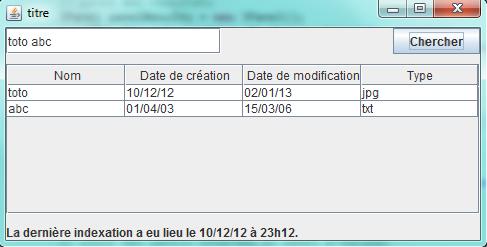
\includegraphics[scale=0.7]{rechercheSimple.png}
\caption{Interface graphique du moteur de recherche.}
\end{figure}

\subsection{Fonctionnalités du produit}
Lors de la première utilisation, iFind lance un démon ayant pour tâche d'indexer
un corpus ciblé. Ce démon va envoyer l'ensemble des données à indexer
à la base d'indexation, qui construira la base de données utilisée pour les 
recherches. Cette base de données va jouer un rôle clé dans la phase de 
recherche de fichiers.
Un algorithme est appliqué pour identifier dans le corpus (en utilisant 
l'index), les fichiers
qui correspondent le mieux aux mots contenus dans la requête, afin de présenter
les résultats des recherches par ordre de pertinence. 
Ensuite, tous les dix évènements détectés par le démon, celui-ci
envoie les nouvelles informations à indexer à la base d'indexation.

\subsubsection{Utilisation normale}
L'utilisateur entre une requête dans la barre de recherche en suivant la syntaxe
du moteur de recherche (cf partie 2.3.2).\\
TODO (retour de la requête)


\subsubsection{Utilisation avancée}

La recherche avancée permet d'affiner la recherche de document en se basant sur un critère de type.
Un utilisateur pourra rechercher des morceaux de musique par artiste, album ou titre du morceaux.
Il pourra aussi recherches des images. Le moteur de recherche dans ce cas cherche à filtrer les résultats pour faire en sorte que
les résultats affichés en sortie corresponde juste à des fichiers de type image. (jpg,jpeg,bmp)

Concernant les documents textuelles, l'interface de recherche de ces documents permet de rechercher un document par auteur du document, genre, extension et la date de modification. La pertinence des résultats obtenus dans ce cas depend de la disponibilité de ce information par rapport a ces documents. C'est à dire, si un genre de document n'est par fourni, et on souhaite rechercher un genre précis du documents.

Il y a des chances que le moteur de recherche ne puisse pas retrouver le document recherché même si celui ci existe sur le disque.

Dans le cas où le document recherché n'est pas présent, un message apparaîtra afin de guider l'utilisateur. 
De plus, la date et l'heure de la dernière indexation est indiqué.

La partie inférieure de la fenêtre permet de visualiser la liste des documents trouvés. 
Cette dernière se compose d'une colonne indiquant le nom du document, une deuxième indiquant sa date de création, une troisième indiquant sa date de modification (la plus récente) et enfin la dernière indiquant le type.



L'utilisateur peut également entrer une requête incluant des critères spéciaux
sur les fichiers à rechercher :
\begin{itemize}
 \item l'auteur
 \item la date de création
 \item la dernière date de modification
 \item le type
 \item la taille (pour les fichiers de type image)
 \item la durée (pour les fichiers de type musique ou vidéo)
\end{itemize}

Il est possible de paramétrer les fonctionnalités suivantes de l'indexation :
\begin{itemize}
 \item Indexation ciblée : on délimite l'emplacement du corpus à indexer.
 \item Indexation filtrée : on peut choisir le type de fichier à indexer.
\end{itemize}


\subsection{Caractéristique d'utilisation}

\subsubsection{Grammaire BNF}
Dans ce paragraphe, on introduira la grammaire qui définira le langage de requêtes que l'on associe au moteur de recherche.\\

Un mot est formé de chiffres et/ou de lettres minuscules ou majuscules, possiblement accentuées.\\

Une requête doit obligatoirement commencer par un mot.\\

Dans le cas d'une recherche multiple, la liste de mots à rechercher est soit délimitée par 
des espaces (dans le cas d'une conjonction), soit délimitée par le marqueur \textbf{-or} (dans le
cas d'une disjonction).\\

La requête peut être complétée par des options :
\begin{itemize}
 \item la recherche par type de fichiers, avec le marqueur \textbf{-f}
 \item l'exclusion d'une liste de mots, avec le marqueur \textbf{-e}
 \end{itemize}

\paragraph{Grammaire BNF\\}
Dans la suite, les symboles terminaux seront notés en \textbf{gras}.
Les symboles non-terminaux seront notés en \textit{italique}. Une séquence entre crochets est optionnelle (comme par exemple ``\textit{[} word \textit{]}'').\\
Une séquence entre accolades se répète zéro fois ou plus, (comme par exemple ``\textit{\{} , word \textit{\}}'').\\
Sauf indication contraire, la sémantique d’une séquence est une liste dont la tête est le premier élément de la séquence.\\

\begin{tabular}{p{1.5cm} p{0.5cm} p{9cm} }
& & \\
\textbf{char} & $\equiv$ & [:alnum:]\\
\textbf{word} & $\equiv$ & $\textbf{char}^+$\\
\textit{query} & ::= & \textbf{word} \textit{\{} \textbf{-or} \textbf{word} \textit{\}} \textit{[} \textit{options} \textit{]}\\
& | & \textbf{word} \textit{\{} \textbf{word} \textit{\}} \textit{[} \textit{options} \textit{]}\\
\textit{options} & ::= & \textbf{-e} \textbf{word} \textit{\{} \textbf{word} \textit{\}}\\
\end{tabular}

% insertion du tableau contenant la syntaxe
\section{Syntaxe MR}

\begin{center}
\begin{tabular}{| p{5cm} | p{8cm} |}
\hline
Minuscules/ majuscules & iFind ne tient pas compte de la casse des caractères.
Les requêtes 'ibm', 'Ibm' et 'IBM' renvoient le même résultat.\\
\hline
Lettres accentuées & \textbf{Important} \textit{electricite} et \textit{électricité}
ne donnent pas le même résultat, même si les différences sont souvent minimes.\\
\hline
<<<<<<< HEAD
Ordre des mots & \textbf{Important}: \textit{paris brest} donne un résultat 
différent de \textit{brest paris}. Une plus grande importance est donnée au premier 
mot choisi.\\
\hline
 Disjonction : Rechercher un mot ou  l'autre, requête -or requête
&
-or
Exemple : machin OR bidon. L'opérateur doit être saisi avec un tiret obligatoirement.\\
\hline
 Conjonction
 ET
& Opérateur par défaut
Exemple : 'moteur recherche' recherche les fichiers qui contiennent à la fois 'moteur' ET 'recherche'. 
Il est également possible d'utiliser le signe + pour demander une orthographe spécifique:
Exemple : +jéremie ne trouvera pas la forme "jeremie" (non accentuée)\\
\hline
 Exclure un mot
-e requête
&-e
Exemple : moteur –e automobile recherche les fichiers qui contiennent 'moteur' mais qui ne contiennent pas automobile.\\
=======
Ordre des mots & \textbf{Important}: \textit{paris brest } donne un résultat 
différent de \textit{brest paris}. Une plus grande importance est donnée au premier 
mot choisi.\\
\hline
Disjonction : Rechercher un mot ou  l'autre, requête -or requête
-or
Exemple : “machin OR bidon”. L'opérateur doit être saisi avec un tiret obligatoirement.
\hline
Conjonction
ET
Opérateur par défaut
Exemple : 'moteur recherche' recherche les fichiers qui contiennent à la fois 'moteur' ET 'recherche'. Il est également possible d'utiliser le signe + pour demander une orthographe spécifique :
Exemple : +jéremie ne trouvera pas la forme 'jeremie (non accentuée)
\hline
 Exclure un mot
-e requête
-e
Exemple : moteur –e automobile recherche les fichiers qui contiennent moteur mais qui ne contiennent pas automobile.
>>>>>>> ef841992d5df638244c7e73e4d6758b1363e056a
\hline
 Expressions & Non. Il n'est pas possible de faire des recherches de phrases exactes.\\
\hline
<<<<<<< HEAD
Troncature & Non. Il n'est pas possible de faire des recherches en utilisant la troncature sur iFind. 
le moteur recherche toujours exactement le mot demandé. 'mot' ne trouve pas 'mots' ni 'moteur'. L'astérique (*) ne peut pas être utilisé. 
iFind tient cependant parfois compte de la troncature, sans qu'il soit possible pour l'utilisateur de décider quand.\\
\hline
 Recherche sur le type de fichier
& -f
Exemple : exemples –f pdf. Plusieurs formats sont possibles.\\
\hline
 Recherche avancée & 
Advanced Search, Recherche avancée
Recherche sur le format de fichiers, sur la date de mise à jour, etc. Cependant, il n’y aura pas de syntaxe spécifique mais des boites de choix au niveau de l’interface graphique.\\
\hline
=======
Troncature
Non
Il n'est pas possible de faire des recherches en utilisant la troncature sur iFind. le moteur recherche toujours exactement le mot demandé. mot ne trouve pas mots ni moteur. L'astérique (*) ne peut pas être utilisé. iFind tient cependant parfois compte de la troncature, sans qu'il soit possible pour l'utilisateur de décider quand.
\hline
 Recherche sur le type   de fichier
-f
Exemple : exemples –f pdf. Plusieurs formats sont possibles.
\hline
 Recherche avancée
Advanced Search, Recherche avancée
Recherche sur le format de fichiers, sur la date de mise à jour, etc. Cependant, il n’y aura pas de syntaxe spécifique mais des boites de choix au niveau de l’interface graphique.

>>>>>>> ef841992d5df638244c7e73e4d6758b1363e056a

\end{tabular}
 
\end{center}



\subsubsection{Messages d'erreur possibles}
Si la requête entrée par l'utilisateur est mal formée, le message suivant apparaît :
"La requête entrée ne respecte pas la syntaxe. Cliquez sur Aide pour plus d'informations."
(Cliquer sur Aide ouvre une petite fenêtre contenant les règles de syntaxe d'une requête.)
L'utilisateur est alors invité à reformuler sa requête.

Si la base de données est corrompue et entraîne l'arrêt de la recherche et de l'indexation, l'utilisateur est invité à la réinitialiser :
"La base de données a été corrompue et doit être intégralement reconstruite. 
Cette opération peut prendre du temps. Voulez-vous réinitialiser la base de données maintenant ?
Si vous cliquez sur Annuler, la base de données ne sera pas reconstruite et iFind ne sera plus utilisable."
((OK) (Annuler) <- boutons)

\subsection{Contraintes générales}
La fraîcheur des résultats dépendra de la fraîcheur de la dernière indexation faite.\\
L'indexation a lieu tous les dix évènements (par exemple, dix créations de fichier).
Il peut arriver qu'un fichier supprimé soit retourné comme résultat d'une recherche, 
mais seulement si le fichier a été supprimé il y a moins de dix évènements.

\subsection{Dépendances}
Le logiciel iFind est utilisable sur une distribution GNU/Linux.\\
Il est nécessaire d'installer PostgreSQL pour utiliser le logiciel.\\
JNotify possède une licence GNU LESSER GENERAL PUBLIC LICENSE Version 2.1, February 1999.
\newpage

\section{Spécification du Système}
Cette partie du cahier de charge présentera les trois axes principaux du développement de ifind.
\begin{itemize}
 \item Architecture du système.
 \item Charges du système.
 \item Modèles dy système.
\end{itemize}

\subsection{Architecture du Système}
Ce paragraphe présente un point du vue haut niveau de l'architecture préconisée du système et la distribution de fonctionnalités à travers 
les modules du système.

Notre système se compose de trois sous-systèmes :
\begin{itemize}
 \item Moteur de recherche : Architecture Model View Controler
 \item Moteur d'indexation : Deamon
 \item Base de donnée indexée : Architecture en couche : PostgreSQL
\end{itemize}

\subsubsection{Architecture du Moteur de recherche}
Le moteur de recherche (MR) communique avec la base d'indexation (BI) par l'intermédiaire d'un flux XML au travers d'une Socket.
Le flux XML envoyé par le MR est associé à un identifiant, qui permet de savoir à quelle requête est associée quelle réponse.
L'envoi respecte la DTD (voir annexe).

\paragraph{BNF}
Nous avons défini une syntaxe et à fortiori, une grammaire sous forme BNF.

Grammaire (BNF) :\\
% \begin{tabular}{r c l}
% query &$\rightarrow$ & word { -or word } [options]\\
% query &$\rightarrow$ & word { word } [options] \\
% 	 
% options&$\rightarrow$ &-e word {word}\\
% word   &$\rightarrow$ &char*\\
% char   &$\rightarrow$ & [a-z A-Z 0-9 à é è ë ä ù ï ç]\\ 
% \end{tabular}

\begin{tabular}{p{1.5cm} p{0.5cm} p{9cm} }
& & \\
\textbf{char} & $\equiv$ & [:alnum:]\\
\textbf{word} & $\equiv$ & $\textbf{char}^+$\\
\textit{query} & ::= & \textbf{word} \textit{\{} \textbf{-or} \textbf{word} \textit{\}} \textit{[} \textit{options} \textit{]}\\
& | & \textbf{word} \textit{\{} \textbf{word} \textit{\}} \textit{[} \textit{options} \textit{]}\\
\textit{options} & ::= & \textbf{-e} \textbf{word} \textit{\{} \textbf{word} \textit{\}}\\
\end{tabular}

Par la suite, nous avons défini plusieurs types abstraits de données permettant de modéliser la grammaire.
Un type a forcément une ou plusieurs opérations de construction. 
Chaque type peut présenter des fonctions d'accès et de test ainsi que des constantes.

\paragraph{Type de données abstraites}
En effet, nous avons définit 6 types tels que :

\begin{tabular}{r l}
%\textbf{Type : operateur} & \\
%constantes :& plus, OR et Exclu : operateur
% note (isabelle) La présence des types [conj] et [disj] rend la constante [operateur] inutile.

\textbf{Type : requête} & \\
_construction :& cons-requete-word : word $\rightarrow$ requête\\
& cons-requete-word-options : word * options $\rightarrow$ requête\\ 
& cons-requete-conj : conj $\rightarrow$ requête\\
& cons-requete-conj-options : conj * options $\rightarrow$ requête\\
& cons-requete-disj : disj $\rightarrow$ requête\\
& cons-requete-disj-options : disj * options $\rightarrow$ requête\\
_test :& est-word : requête $\rightarrow$ bool\\
& est-conj : requête $\rightarrow$ bool\\
& est-disj : requête $\rightarrow$ bool\\
& a-options : requête $\rightarrow$ bool\\
% est-valide : requête $\rightarrow$ bool\\
% note (isabelle) une requête qui est construite est par définition valide (sauf erreur de ma part), donc ce test est inutile.
_accès :& get-word : requête $\rightarrow$ word\\
& get-conj : requête $\rightarrow$ conj\\
& get-disj : requête $\rightarrow$ disj\\
& get-options : requête $\rightarrow$ options\\
\end{tabular}

\paragraph{}
On garde get-conj() si est conj : get-word() puis recherche conjonction et
get-disj() si est disj : get-word() puis recherche disjonction.
\paragraph{}

\begin{tabular}{r l}
\textbf{Type : conj} &\\
_construction :& cons-conj : word * conj $\rightarrow$ conj\\
& cons-conj-simple : word * word $\rightarrow$ conj\\
_test :& est-conj : conj $\rightarrow$ bool\\
_accès :& get-head : conj $\rightarrow$ word\\
& get-tail : conj $\rightarrow$ conj\\
& \\

\textbf{Type : disj}&\\
_construction :& cons-disj : word * disj $\rightarrow$ disj\\
& cons-disj-simple : word * word $\rightarrow$ disj\\
& accès : getDisj()\\
& \\

\textbf{Type : word}&\\ 
_construction :& cons_word : string $\rightarrow$ word\\
_accès :& get-word : word $\rightarrow$ string\\
& \\

\textbf{Type : options}&\\
_construction :& cons-options : word $\rightarrow$ options\\
& cons-options-simple : word * word $\rightarrow$ options\\
_test :& est-options : options $\rightarrow$ bool\\
_accès :& get-head : options $\rightarrow$ word\\
& get-tail : options $\rightarrow$ options
\end{tabular}


Model :

View : GUI

Controler : search-engine-core
\begin{center}
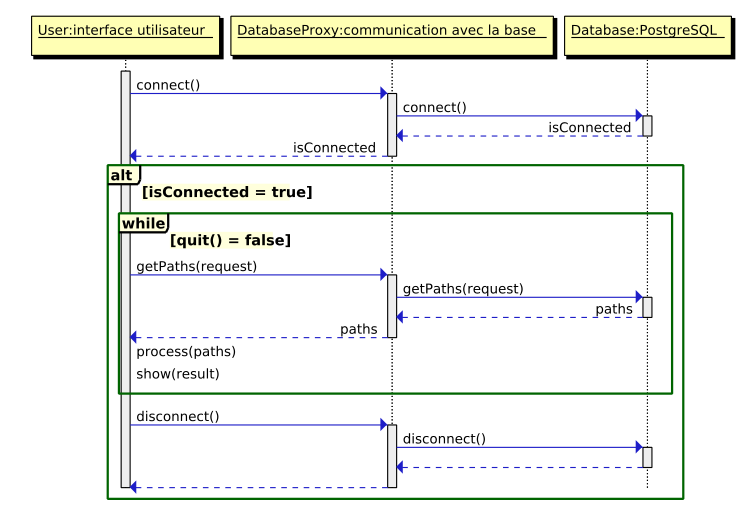
\includegraphics[scale=0.5]{seqmrbi.png}
\end{center}


\subsubsection{Architecture du moteur d'indexation}
Le moteur d'indexation se compose de deux instances.\\
La première est lancée uniquement lorsqu'il faut entièrement créer l'index (lors de l'installation, par exemple).\\
La deuxième, le démon, communique en permanence avec la base d'indexation afin de lui envoyer
les différents évènements qui ont eu lieu à l'intérieur du corpus et qui doivent être indexés.
L'envoi se fait par l'intermédiaire d'un flux XML au travers d'une Socket. L'envoi respecte la DTD (voir annexe)
établie par les chefs de projets pendant les réunions.

\subsubsection{Architecture de la base d'indexation}
La base d'indexation est une base de donnée PostgreSQL, en un premier temps, qui permettra au moteur de recherche 
de retrouver ce qu'il cherche.

\begin{center}
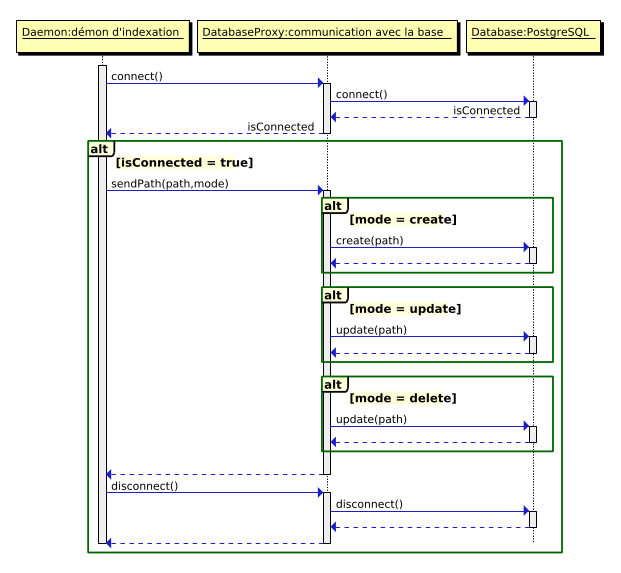
\includegraphics[scale=0.5]{seqdbi.png}
\end{center}

Le modèle conceptuel de données (MCD) de la base de données est le suivant :
\begin{center}
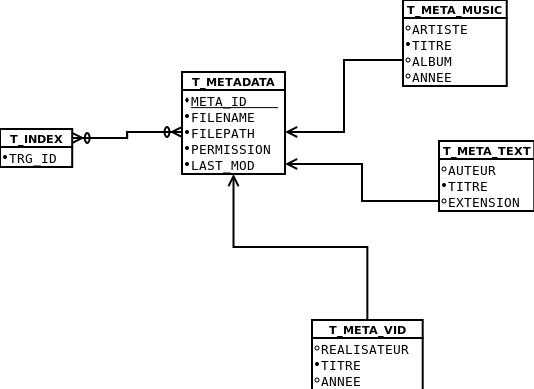
\includegraphics[scale=0.7]{mcd.png}
\end{center}


\subsection{Charges du Système}
Ce paragraphe décrit les charges fonctionnelles du système en détail et d'autres charges non fonctionnelles : 
\begin{itemize}
 \item interface
 \item autres...
\end{itemize}

\subsection{Modèles du système}
Ce paragraphe décrit les divers modèles du système ainsi que leurs relations entre composantes du système et de son environnement.

\subsubsection{Modèle de communication}
Le base d'indexation écoute sur deux ports différents, un pour la communication avec le moteur d'indexation, 
et un pour la communication avec le moteur de recherche.

\paragraph{Communication avec le moteur d'indexation}
La base d'indexation (BI) attend qu'un moteur d'indexation (MI) se connecte sur le port 40000. Lorsque la connexion est établie, 
la BI lit le flux XML envoyé par le MI. La connexion entre le MI et la BI n'est fermée que lorsque l'un des deux modules
est fermé.

\paragraph{Communication avec le moteur de recherche}
La base d'indexation (BI) attend qu'un moteur de recherche (MR) se connecte sur le port 30000. Lorsque la connexion est établie,
la BI lit le flux XML envoyé par le MR. La BI génère une réponse au flux et la renvoie au MR, via le port 30000 sous forme de XML.


\newpage
\section{Annexe}

\subsection{Communication du moteur d'indexation vers la base d'indexation (DTD)}
\begin{verbatim}
<!-- règle génerale :
chaque fichier Xml doit contenir la ligne suivante
<?xml version="1.0" encoding="UTF-8"?> -->

<!-- comme convenue toutes les balises de l'indexation sont facultatives -->
<!ELEMENT INDEXATION (RENOMMAGES?, MODIFICATIONS?, SUPPRESSIONS?, CREATIONS?)>

<!ELEMENT RENOMMAGES (FICHIERRENOMME)*>		
<!ELEMENT MODIFICATIONS (FICHIERMODIFIE)*>	
<!ELEMENT SUPPRESSIONS (FICHIERSUPPRIME)*>
<!ELEMENT CREATIONS (FICHIERCREE)*>		

<!ELEMENT FICHIERRENOMME (PATH, NEWPATH)>
<!-- un fichier renommé n'est pas nécessairement un fichier modifié -->
<!-- un fichier modifé nécessite une re-indexation --> 
<!ELEMENT FICHIERMODIFIE (PATH, DATEMODIFICATION, TAILLE, PROPRIETAIRE, GROUPE, 
PERMISSIONS, INDEXAGE, NEWPATH?)>
<!ELEMENT FICHIERSUPPRIME (PATH)>
<!ELEMENT FICHIERCREE (PATH, format, DATECREATION, TAILLE, PROPRIETAIRE, GROUPE, 
PERMISSIONS, INDEXAGE)>

<!-- les meta-données --> 
<!ELEMENT PATH (#PCDATA)>
<!ELEMENT format (#PCDATA)>
<!ELEMENT DATECREATION (#PCDATA)>
<!ELEMENT DATEMODIFICATION (#PCDATA)>
<!ELEMENT TAILLE (#PCDATA)>
<!ELEMENT PROPRIETAIRE (#PCDATA)>
<!ELEMENT GROUPE (#PCDATA)>
<!ELEMENT PERMISSIONS (#PCDATA)>
<!-- liste des mots a indexer -->
<!ELEMENT INDEXAGE (MOT*)>
<!ELEMENT MOT (#PCDATA)><!ATTLIST MOT frequence CDATA #REQUIRED>
<!ELEMENT NEWPATH (#PCDATA)>

<!-- les id's seront utlisés pour la traçabilitée et la détection d'eventuel 
erreurs, elle sont tout de même facultatives --> 
<!ATTLIST RENOMMAGES id CDATA #IMPLIED>
<!ATTLIST MODIFICATIONS id CDATA #IMPLIED>
<!ATTLIST SUPPRESSIONS id CDATA #IMPLIED>
<!ATTLIST CREATIONS id CDATA #IMPLIED>
\end{verbatim}

\subsection{Communication du moteur de recherche vers le moteur d'indexation (DTD)}
\begin{verbatim}
 <!-- Description de la requête de recherche -->
<!ELEMENT SEARCH (WORD, CONTENT?, PATHDIR?, PERM?, EXTENSION?, TIMESLOT?)>
<!-- Le mot à rechercher -->
<!ELEMENT WORD (#PCDATA)>
<!-- Un booléen qui dit si l'on fait une recherche de contenu (true) ou une 
recherche sur les nom de fichier (false) -->
<!ELEMENT CONTENT (#PCDATA)>
<!-- Le nom du fichier à partir duquel on recherche -->
<!ELEMENT PATHDIR (#PCDATA)>
<!-- Les permissions du fichier à chercher -->
<!ELEMENT PERM (#PCDATA)>
<!-- L'extension des fichiers à chercher -->
<!ELEMENT EXTENSION (#PCDATA)>
<!-- Interval de temps -->
<!ELEMENT TIMESLOT (BEGIN, END)>
<!-- Debut de l'interval -->
<!ELEMENT BEGIN (DAY, MONTH, YEAR)>
<!-- Fin de l'interval -->
<!ELEMENT END (DAY, MONTH, YEAR)>
<!-- Le jour -->
<!ELEMENT DAY (#PCDATA)>
<!-- Le mois -->
<!ELEMENT MONTH (#PCDATA)>
<!-- L'année -->
<!ELEMENT YEAR (#PCDATA)>

<!-- L'id du resultat correspondant à une recherche aura le même id que la 
recherche -->
<!ATTLIST SEARCH id CDATA #REQUIRED>
\end{verbatim}

\subsection{Communication de la base d'indexation vers le moteur de recherche (DTD)}
\begin{verbatim}
 <!-- Balise contenant les résultats de la requête search -->
<!ELEMENT RESULT (FILE*)>
<!-- Balise file correspond à un fichier resultat donc n balises files = n 
résultats -->
<!ELEMENT FILE (NAME, PATH, PERM, SIZE, LASTMODIF?, PROPRIO?)>
<!-- Le nom du fichier -->
<!ELEMENT NAME (#PCDATA)>
<!-- Le chemin complet du fichier -->
<!ELEMENT PATH (#PCDATA)>
<!-- Les permissions du fichier -->
<!ELEMENT PERM (#PCDATA)>
<!-- La taille du fichier -->
<!ELEMENT SIZE (#PCDATA)>
<!-- La date de dérnière modification du fichier -->
<!ELEMENT LASTMODIF (#PCDATA)>
<!-- Le propriétaire du fichier -->
<!ELEMENT PROPRIO (#PCDATA)>

<!-- L'id du resultat correspondant à une recherche aura le même id que la 
recherche -->
<!ATTLIST RESULT id CDATA #REQUIRED>
\end{verbatim}
